\documentclass[fleqn,10pt]{article}
\usepackage[utf8]{inputenc}
\usepackage[T1]{fontenc}

\usepackage[margin=2.5cm, includefoot, footskip=30pt]{geometry}
\pagestyle{plain}
\setlength{\parindent}{0em}
\setlength{\parskip}{1em}
\renewcommand{\baselinestretch}{1}

\usepackage{amsmath}
\usepackage{amssymb}
\usepackage{mathtools}
\usepackage{amsthm}
\newcommand{\R}{\mathbb{R}}
\newtheorem{theorem}{Theorem}
\newtheorem{lemma}[theorem]{Lemma}

\usepackage{setspace}
\usepackage{authblk}


\title{Supplementary Information: A theory of mind: Best responses to memory-one strategies. The limitations
of extortion and restricted memory}

\author[1,2,*]{Nikoleta E. Glynatsi}
\author[1]{Vincent A. Knight}
\affil[1]{Cardiff University, School of Mathematics, Cardiff, CF24 4AG, United Kingdom}
\affil[2]{Max Planck Institute for Evolutionary Biology, Pl\"{o}n, 24 306, Germany}

\affil[*]{glynatsi@evolbio.mpg.de}

\date{}

\begin{document}
\maketitle

\section{Theorem~1 Proof}\label{appendix:theorem_one}

The utility of a memory one player \(p\) against an opponent \(q\), \(u_q(p)\),
can be written as a ratio of two quadratic forms on \(R^4\).

\begin{proof}

    It was discussed that \(u_q(p)\) it is the product of the steady state
    vector \(v\) and the PD payoffs,

    \[u_q(p) = v \cdot (R, S, T, P).\]

    The steady state vector which is the solution to \(vM = v\) is given by
    \begingroup
    \tiny
    \begin{equation*}
    \begin{split}
        v =  & \left[ \frac{p_{2} p_{3} (q_{2} q_{4} - q_{3} q_{4}) + p_{2} p_{4} (q_{2} q_{3} - q_{2} q_{4} - q_{3} + q_{4}) +
        p_{3} p_{4} (- q_{2} q_{3} + q_{3} q_{4}) - p_{3} q_{2} q_{4} + p_{4}q_{4} (q_{2} - 1)}{\bar{v}} \right., \\
        & \left. \frac{p_{1} p_{3} (q_{1} q_{4} - q_{2} q_{4}) + p_{1} p_{4} (- q_{1} q_{2} + q_{1} + q_{2} q_{4} -
        q_{4}) + p_{3} p_{4} (q_{1} q_{2} - q_{1} q_{4} - q_{2} + q_{4}) + p_{3}q_{4} (q_{2} - 1) -
         p_{4} q_{2} (q_{4} + 1) + p_{4} (q_{4} - 1)}{\bar{v}} \right., \\
        & \left. \frac{- p_{1} p_{2} (q_{1} q_{4} - q_{3} q_{4}) - p_{1} p_{4} (- q_{1} q_{3} + q_{3} q_{4})
          + p_{1} q_{1} q_{4} - p_{2} p_{4} (q_{1} q_{3} - q_{1} q_{4} - q_{3} + q_{4}) -
          p_{2} q_{4} (q_{3}  + 1) - p_{4}q_{4} (q_{1} + q_{3}) - p_{4} (q_{3}
          + q_{4}) - q_{4}}{\bar{v}} \right., \\ 
        & \left. \frac{p_{1} p_{2} (q_{1} q_{2} - q_{1} - q_{2} q_{3} + q_{3}) + p_{1} p_{3} (- q_{1} q_{3} + q_{2} q_{3})
         - p_{1} q_{1} (q_{2} + 1) + p_{2} p_{3} (- q_{1} q_{2} + q_{1} q_{3}
         + q_{2} - q_{3}) + p_{2} (q_{3}q_{2}  - q_{2} - q_{3} - 1) +
          p_{3} (q_{1} q_{2} - q_{3}q_{2} - q_{2} - q_{3}) + q_{2} - 1}{\bar{v}}\right],
    \end{split}
    \end{equation*}
    \endgroup

    where,
    \begingroup
    \footnotesize
    \begin{equation*}
        \begin{split}
           \bar{v} = & \quad p_{1} p_{2} (q_{1} q_{2} - q_{1} q_{4} - q_{1} - q_{2} q_{3} + q_{3} q_{4} + q_{3}) - p_{1} p_{3} (q_{1} q_{3} - q_{1} q_{4} - q_{2} q_{3} + q_{2} q_{4}) -
           p_{1} p_{4} (q_{1} q_{2} - q_{1} q_{3} - q_{1} - q_{2} q_{4} + q_{3} q_{4} + q_{4}) - \\
           & \quad p_{1} q_{1} (q_{2} + q_{4} + 1) + p_{2} p_{3} (- q_{1} q_{2} + q_{1} q_{3} + q_{2} q_{4} + q_{2} - q_{3} q_{4} - q_{3})
           + p_{2} p_{4} (- q_{1} q_{3} + q_{1} q_{4} + q_{2} q_{3} - q_{2} q_{4}) + p_{2} q_{2} (q_{3} - 1) - p_{2} q_{3} (q_{4} - 1) + \\
           & \quad p_{2} (q_{4} + 1) +  p_{3} p_{4} (q_{1} q_{2} - q_{1} q_{4} - q_{2} q_{3} - q_{2} + q_{3} q_{4} + q_{4}) + p_{3} q_{2} q_{1} ( - p_{3} - 1) + p_{3} (q_{3} -
           q_{4}) - p_{4} (q_{1} q_{4} + q_{2} + q_{3} q_{4} - q_{3} + q_{4} - 1) + \\
           & \quad q_{2} - q_{4} - 1
        \end{split}
        \end{equation*}
    \endgroup

    The dot product of \(v \cdot (R, S, T, P)\) gives,

    \begingroup
    \scriptsize
    \begin{equation*}
    \begin{split}
        u_q(p) = & \frac{R \left(p_{2} p_{3} (q_{2} q_{4} - q_{3} q_{4}) + p_{2} p_{4} (q_{2} q_{3} - q_{2} q_{4} - q_{3} + q_{4}) +
        p_{3} p_{4} (- q_{2} q_{3} + q_{3} q_{4}) - p_{3} q_{2} q_{4} + p_{4}q_{4} (q_{2} - 1)\right)}{\bar{v}}  +  \\
        & \frac{S \left(p_{1} p_{3} (q_{1} q_{4} - q_{2} q_{4}) + p_{1} p_{4} (- q_{1} q_{2} + q_{1} + q_{2} q_{4} -
        q_{4}) + p_{3} p_{4} (q_{1} q_{2} - q_{1} q_{4} - q_{2} + q_{4}) + p_{3}q_{4} (q_{2} - 1) -
         p_{4} q_{2} (q_{4} + 1) + p_{4} (q_{4} - 1)\right)}{\bar{v}} + \\
        & \frac{T \left(- p_{1} p_{2} (q_{1} q_{4} - q_{3} q_{4}) - p_{1} p_{4} (- q_{1} q_{3} + q_{3} q_{4})
          + p_{1} q_{1} q_{4} - p_{2} p_{4} (q_{1} q_{3} - q_{1} q_{4} - q_{3} + q_{4}) -
          p_{2} q_{4} (q_{3}  + 1) - p_{4}q_{4} (q_{1} + q_{3}) - p_{4} (q_{3}
          + q_{4}) - q_{4}\right)}{\bar{v}} + \\ 
        & \frac{P \left(p_{1} (p_{2} (q_{1} q_{2} - q_{1} - q_{2} q_{3} + q_{3}) + p_{3} (- q_{1} q_{3} + q_{2} q_{3})
        - q_{1} (q_{2} + 1)) + p_{2} p_{3} ((- q_{1} q_{2} + q_{1} q_{3}
        + q_{2} - q_{3}) + (q_{3}q_{2}  - q_{2} - q_{3} - 1))\right)}{\bar{v}} + \\
        & \frac{P \left(p_{3} (q_{1} q_{2} - q_{3}q_{2} - q_{2} - q_{3}) + q_{2} - 1\right)}{\bar{v}} \implies \\
    \end{split}
    \end{equation*}
    \endgroup

    \begingroup
    \scriptsize
    \begin{equation*}
        u_q(p) =
        \left(
          \frac
            {\parbox{6in}{$ - p_{1} p_{2} (q_{1} - q_{3}) (P q_{2} - P - T q_{4}) + p_{1} p_{3} (q_{1} - q_{2}) (P q_{3} - S q_{4}) + p_{1} p_{4} (q_{1} - q_{4}) (S q_{2} - S - T q_{3}) + p_{2} p_{3} (q_{2} - q_{3}) (P q_{1} - P - R q_{4}) - $ \\
            $ p_{2} p_{4} (q_{3} - q_{4}) (R q_{2} - R - T q_{1} + T) + p_{3} p_{4} (q_{2} - q_{4}) (R q_{3} - S q_{1} + S) + p_{1} q_{1} (P q_{2} - P - T q_{4}) - p_{2} (q_{3} - 1) (P q_{2} - P - T q_{4}) + $ \\
            $ p_{3} (- P q_{1} q_{2} + P q_{2} q_{3} + P q_{2} - P q_{3} + R q_{2} q_{4} - S q_{2} q_{4} + S q_{4}) + p_{4} (- R q_{2} q_{4} + R q_{4} + S q_{2} q_{4} - S q_{2} - S q_{4} + S + T q_{1} q_{4} - T q_{3} q_{4} + T q_{3} - T q_{4}) $ \\
            \hspace*{6.7cm} $- P q_{2} + P + T q_{4}$
            }}
            {\parbox{6in}{$
            p_{1} p_{2} (q_{1} q_{2} - q_{1} q_{4} - q_{1} - q_{2} q_{3} + q_{3} q_{4} + q_{3}) + p_{1} p_{3} (- q_{1} q_{3} + q_{1} q_{4} + q_{2} q_{3} - q_{2} q_{4}) + p_{1} p_{4} (- q_{1} q_{2} + q_{1} q_{3} + q_{1} + q_{2} q_{4} - q_{3} q_{4} - q_{4}) +$ \\
            $ p_{2} p_{3} (- q_{1} q_{2} + q_{1} q_{3} + q_{2} q_{4} + q_{2} - q_{3} q_{4} - q_{3}) + p_{2} p_{4} (- q_{1} q_{3} + q_{1} q_{4} + q_{2} q_{3} - q_{2} q_{4}) + p_{3} p_{4} (q_{1} q_{2} - q_{1} q_{4} - q_{2} q_{3} - q_{2} + q_{3} q_{4} + q_{4}) + $ \\
            $ p_{1} (- q_{1} q_{2} + q_{1} q_{4} + q_{1}) + p_{2} (q_{2} q_{3} - q_{2} - q_{3} q_{4} - q_{3} + q_{4} + 1) + p_{3} (q_{1} q_{2} - q_{2} q_{3} - q_{2} + q_{3} - q_{4}) + p_{4} (- q_{1} q_{4} + q_{2} + q_{3} q_{4} - q_{3} + q_{4} - 1) + $ \\
            \hspace*{7cm} $q_{2} - q_{4} - 1$
          }}
        \right).
    \end{equation*}
    \endgroup

    Let us consider the numerator of \(u_q(p)\). The cross product terms
    \(p_ip_j\) are given by,

    \begingroup
    \footnotesize
    \begin{align*}
    - p_{1} p_{2} (q_{1} - q_{3}) (P q_{2} - P - T q_{4}) + p_{1} p_{3} (q_{1} - q_{2}) (P q_{3} - S q_{4}) + p_{1} p_{4} (q_{1} - q_{4}) (S q_{2} - S - T q_{3}) + \\
    p_{2} p_{3} (q_{2} - q_{3}) (P q_{1} - P - R q_{4}) - p_{2} p_{4} (q_{3} - q_{4}) (R q_{2} - R - T q_{1} + T) + p_{3} p_{4} (q_{2} - q_{4}) (R q_{3} - S q_{1} + S)
    \end{align*}
    \endgroup

    This can be re written in a matrix format given by
    Equation~(\ref{eq:cross_product_coeffs}).

    \begin{equation}\label{eq:cross_product_coeffs}
        \resizebox{0.9\linewidth}{!}{\arraycolsep=2.5pt%
        \boldmath\(
        (p_1, p_2, p_3, p_4) \frac{1}{2} \left[\begin{matrix}0 & 5 q_{4} \left(q_{1} - q_{3}\right) & - q_{4} \left(q_{1} - q_{2}\right) & \left(q_{1} - q_{4}\right) \left(q_{2} - 5 q_{3} - 1\right)\\5 q_{4} \left(q_{1} - q_{3}\right) & 0 & - 3 q_{4} \left(q_{2} - q_{3}\right) & \left(q_{3} - q_{4}\right) \left(5 q_{1} - 3 q_{2} - 2\right)\\- q_{4} \left(q_{1} - q_{2}\right) & - 3 q_{4} \left(q_{2} - q_{3}\right) & 0 & - \left(q_{2} - q_{4}\right) \left(q_{1} - 3 q_{3} - 1\right)\\\left(q_{1} - q_{4}\right) \left(q_{2} - 5 q_{3} - 1\right) & \left(q_{3} - q_{4}\right) \left(5 q_{1} - 3 q_{2} - 2\right) & - \left(q_{2} - q_{4}\right) \left(q_{1} - 3 q_{3} - 1\right) & 0\end{matrix}\right] \begin{pmatrix}
        p_1 \\
        p_2 \\
        p_3 \\
        p_4 \end{pmatrix}
        \) }
    \end{equation}

    Similarly, the linear terms are given by,

    \begingroup
    \footnotesize
    \begin{align*}
    p_{1} q_{1} (P q_{2} - P - T q_{4}) - p_{2} & (q_{3} - 1) (P q_{2} - P - T q_{4}) + p_{3} (- P q_{1} q_{2} + P q_{2} q_{3} + P q_{2} - P q_{3} + R q_{2} q_{4} - S q_{2} q_{4} + S q_{4}) + \\
    p_{4} & (- R q_{2} q_{4} + R q_{4} + S q_{2} q_{4} - S q_{2} - S q_{4} + S + T q_{1} q_{4} - T q_{3} q_{4} + T q_{3} - T q_{4})
    \end{align*}
    \endgroup

    and the expression can be written using a matrix format as
    Equation~(\ref{eq:linear_coeffs}).

    \begin{equation}\label{eq:linear_coeffs}
        \resizebox{0.60\linewidth}{!}{\arraycolsep=2.5pt%
        \boldmath\(
        (p_1, p_2, p_3, p_4) \left[\begin{matrix}- 5 q_{1} q_{4}\\5 q_{4} \left(q_{3} - 1\right)\\q_{4} \left(2 q_{2} + 1\right)\\5 q_{1} q_{4} - 2 q_{2} q_{4} - q_{2} - 5 q_{3} q_{4} + 5 q_{3} - 3 q_{4} + 1\end{matrix}\right]\)}
    \end{equation}

    Finally, the constant term of the numerator, which is obtained by
    substituting $p=(0, 0, 0, 0)$, is given by Equation~(\ref{eq:constant}).

    \begin{equation}\label{eq:constant}
    - P q_{2} + P + T q_{4}
    \end{equation}

    Combining Equation~(\ref{eq:cross_product_coeffs}), Equation~(\ref{eq:linear_coeffs}) and
    Equation~(\ref{eq:constant}) gives that the numerator of \(u_q(p)\) can be written
    as,

    \begingroup
    \tiny\boldmath
    \begin{align*}
        \frac{1}{2}p & \left[\begin{matrix}0 & 5 q_{4} \left(q_{1} - q_{3}\right) & - q_{4} \left(q_{1} - q_{2}\right) & \left(q_{1} - q_{4}\right) \left(q_{2} - 5 q_{3} - 1\right)\\5 q_{4} \left(q_{1} - q_{3}\right) & 0 & - 3 q_{4} \left(q_{2} - q_{3}\right) & \left(q_{3} - q_{4}\right) \left(5 q_{1} - 3 q_{2} - 2\right)\\- q_{4} \left(q_{1} - q_{2}\right) & - 3 q_{4} \left(q_{2} - q_{3}\right) & 0 & - \left(q_{2} - q_{4}\right) \left(q_{1} - 3 q_{3} - 1\right)\\\left(q_{1} - q_{4}\right) \left(q_{2} - 5 q_{3} - 1\right) & \left(q_{3} - q_{4}\right) \left(5 q_{1} - 3 q_{2} - 2\right) & - \left(q_{2} - q_{4}\right) \left(q_{1} - 3 q_{3} - 1\right) & 0\end{matrix}\right] p^T +  \\
        & \left[\begin{matrix}- 5 q_{1} q_{4}\\5 q_{4} \left(q_{3} - 1\right)\\q_{4} \left(2 q_{2} + 1\right)\\5 q_{1} q_{4} - 2 q_{2} q_{4} - q_{2} - 5 q_{3} q_{4} + 5 q_{3} - 3 q_{4} + 1\end{matrix}\right] p - P q_{2} + P + T q_{4}
    \end{align*}
    \endgroup

    and equivalently as,

    \[\frac{1}{2}pQp^T + cp + a\]

    where \(Q\) \(\in \R^{4\times4}\) is a square matrix defined by the
    transition probabilities of the opponent \(q_1, q_2, q_3, q_4\) as follows:

    \begin{equation*}
        \resizebox{0.9\linewidth}{!}{\arraycolsep=2.5pt%
        \boldmath\(
        Q = \left[\begin{matrix}0 & 5 q_{4} \left(q_{1} - q_{3}\right) & - q_{4} \left(q_{1} - q_{2}\right) & \left(q_{1} - q_{4}\right) \left(q_{2} - 5 q_{3} - 1\right)\\5 q_{4} \left(q_{1} - q_{3}\right) & 0 & - 3 q_{4} \left(q_{2} - q_{3}\right) & \left(q_{3} - q_{4}\right) \left(5 q_{1} - 3 q_{2} - 2\right)\\- q_{4} \left(q_{1} - q_{2}\right) & - 3 q_{4} \left(q_{2} - q_{3}\right) & 0 & - \left(q_{2} - q_{4}\right) \left(q_{1} - 3 q_{3} - 1\right)\\\left(q_{1} - q_{4}\right) \left(q_{2} - 5 q_{3} - 1\right) & \left(q_{3} - q_{4}\right) \left(5 q_{1} - 3 q_{2} - 2\right) & - \left(q_{2} - q_{4}\right) \left(q_{1} - 3 q_{3} - 1\right) & 0\end{matrix}\right]\)},
    \end{equation*}

    \(c\) \(\in \R^{4 \times 1}\) is similarly defined by:

    \begin{equation*}
        \resizebox{0.55\linewidth}{!}{\arraycolsep=2.5pt%
        \boldmath\(c = \left[\begin{matrix}- 5 q_{1} q_{4}\\5 q_{4} \left(q_{3} - 1\right)\\q_{4} \left(2 q_{2} + 1\right)\\5 q_{1} q_{4} - 2 q_{2} q_{4} - q_{2} - 5 q_{3} q_{4} + 5 q_{3} - 3 q_{4} + 1\end{matrix}\right]\),}
    \end{equation*}

    and \(a = 5 q_{4}\).

    The same process is done for the denominator.
\end{proof}

\section{Theorem~2 Proof}\label{appendix:memone_group_best_response}

The optimal behaviour of a memory-one strategy player \(p^* \in \R_{[0, 1]} ^
4\) against a set of \(N\) opponents \(\{q^{(1)}, q^{(2)}, \dots, q^{(N)} \}\)
for \(q^{(i)} \in \R_{[0, 1]} ^ 4\) is given by:

\[p^* = \textnormal{argmax}\sum\limits_{i=1} ^ N  u_q(p), \ p \in S_q.\]

The set \(S_q\) is defined as all the possible combinations of:

\begin{equation}\label{eq:s_q_set}
    S_q =
    \left\{p \in \mathbb{R} ^ 4 \left|
        \begin{aligned}
            \bullet\quad p_j \in \{0, 1\} & \quad \text{and} \quad \frac{d}{dp_k}
            \sum\limits_{i=1} ^ N  u_q^{(i)}(p) = 0 \\
            & \quad \text{for all} \quad j \in J \quad \&  \quad k \in K  \quad \text{for all} \quad J, K \\
            & \quad \text{where} \quad J \cap K = \O \quad
            \text{and} \quad J \cup K = \{1, 2, 3, 4\}.\\
            \bullet\quad  p \in \{0, 1\} ^ 4
        \end{aligned}\right.
    \right\}.
\end{equation}

\begin{proof}
    The optimisation problem of Equation~(\ref{eq:mo_tournament_optimisation})

    \begin{equation}\label{eq:mo_tournament_optimisation}
        \begin{aligned}
        \max_p: & \ \sum_{i=1} ^ {N} {u_q}^{(i)} (p)
        \\
        \text{such that}: & \ p \in \R_{[0, 1]}
        \end{aligned}
    \end{equation}

    can be written as:

    \begin{equation}\label{eq:mo_tournament_optimisation_standard}
        \begin{aligned}
        \max_p: & \ \sum_{i=1} ^ {N} {u_q}^{(i)} (p)
        \\
        \text{such that}: p_i & \leq 1 \text{ for } \in \{1, 2, 3, 4\} \\
        - p_i & \leq 0 \text{ for } \in \{1, 2, 3, 4\} \\
        \end{aligned}
    \end{equation}

    The optimisation problem has two inequality constraints and regarding the
    optimality this means that:

    \begin{itemize}
        \item either the optimum is away from the boundary of the optimization
        domain, and so the constraints plays no role;
        \item or the optimum is on the constraint boundary.
    \end{itemize}

    Thus, the following three cases must be considered:

    \textbf{Case 1:} The solution is on the boundary and any of the possible
    combinations for $p_i \in \{0, 1\}$ for $i \in \{1, 2, 3, 4\}$ are candidate
    optimal solutions.

    \textbf{Case 2:} The optimum is away from the boundary of the optimization
    domain and the interior solution $p^*$ necessarily satisfies the condition
    \(\frac{d}{dp} \sum\limits_{i=1} ^ N  u_q(p^*) = 0\).

    \textbf{Case 3:} The optimum is away from the boundary of the optimization
    domain but some constraints are equalities. The candidate solutions in this
    case are any combinations of $p_j \in \{0, 1\} \quad \text{and} \quad
    \frac{d}{dp_k} \sum\limits_{i=1} ^ N  u_q^{(i)}(p) = 0$ forall $ j \in J
    \text{ \& } k \in K \text{ forall } J, K \text{ where } J \cap K = \O
    \text{ and } J \cup K = \{1, 2, 3, 4\}.$

    Combining cases 1-3 a set of candidate solutions, denoted as \(S_q\), is
    constructed as: {\scriptsize
    \begin{equation*}
        S_q =
        \left\{p \in \mathbb{R} ^ 4 \left|
            \begin{aligned}
                \bullet\quad p_j \in \{0, 1\} & \quad \text{and} \quad \frac{d}{dp_k}
                \sum\limits_{i=1} ^ N  u_q^{(i)}(p) = 0
                \quad \text{for all} \quad j \in J \quad \&  \quad k \in K  \quad \text{for all} \quad J, K \\
                & \quad \text{where} \quad J \cap K = \O \quad
                \text{and} \quad J \cup K = \{1, 2, 3, 4\}.\\
                \bullet\quad  p \in \{0, 1\} ^ 4
            \end{aligned}\right.
        \right\}.
    \end{equation*}}

    The derivative of \(\sum\limits_{i=1} ^ N  u_q^{(i)}(p)\) calculated using
    the following property (see~\cite{Abadir2005} for details):

    \begin{equation}\label{eq:first_derivative_property}
    \frac{d x A x^T}{dx} =  2Ax.
    \end{equation}

    Using property~(\ref{eq:first_derivative_property}):

    \begin{equation}\label{eq:quadratics_derivatives}
    \frac{d}{dp} \frac{1}{2}pQp^T + cp + a = pQ + c \text{ and } \frac{d}{dp} \frac{1}{2}p\bar{Q}p^T + \bar{c}p + \bar{a} = p\bar{Q} + \bar{c}.
    \end{equation}

    Note that the derivative of \(cp\) is \(c\) and the constant disappears.
    Combining these it can be proven that:

    \begingroup
    \footnotesize
    \begin{align*}
    \frac{d}{dp} \sum\limits_{i=1} ^ N  u_q^{(i)}(p) & = \sum\limits_{i=1} ^ N \frac{\frac{d}{dp}(\frac{1}{2}pQ^{(i)}p^T + c^{(i)}p + a^{(i)} )(\frac{1}{2}p\bar{Q^{(i)}}p^T + \bar{c^{(i)}}p + \bar{a^{(i)}}) -
    \frac{d}{dp}(\frac{1}{2}p\bar{Q^{(i)}}p^T + \bar{c^{(i)}}p + \bar{a^{(i)}})(\frac{1}{2}pQ^{(i)}p^T + c^{(i)}p + a^{(i)})}{(\frac{1}{2}p\bar{Q^{(i)}}p^T + \bar{c^{(i)}}p + \bar{a^{(i)}})^2} \\
    & = \sum\limits_{i=1} ^ N \frac{(pQ^{(i)} + c^{(i)} +)(\frac{1}{2}p\bar{Q^{(i)}}p^T + \bar{c^{(i)}}p + \bar{a^{(i)}})}{(\frac{1}{2}p\bar{Q^{(i)}}p^T + \bar{c^{(i)}}p + \bar{a^{(i)}})^2} -
     \frac{(p\bar{Q^{(i)}}+ \bar{c^{(i)}})(\frac{1}{2}pQ^{(i)}p^T + c^{(i)}p + a^{(i)})}{(\frac{1}{2}p\bar{Q^{(i)}}p^T + \bar{c^{(i)}}p + \bar{a^{(i)}})^2}
    \end{align*}
    \endgroup

    For \(\frac{d}{dp} \sum\limits_{i=1} ^ N  u_q(p)\) to equal zero then:

    \begin{align}\label{eq:polynomials_roots}
        \displaystyle\sum\limits_{i=1} ^ {N}
        \left(pQ^{(i)} + c^{(i)}\right) \left(\frac{1}{2} p\bar{Q}^{(i)} p^T + \bar{c}^{(i)} p + \bar{a}^ {(i)}\right)
        - \left(p\bar{Q}^{(i)} + \bar{c}^{(i)}\right) \left(\frac{1}{2} pQ^{(i)} p^T + c^{(i)} p + a^ {(i)}\right)
        & = 0, \quad {while} \\
        \displaystyle\sum\limits_{i=1} ^ {N} \frac{1}{2} p\bar{Q}^{(i)} p^T + \bar{c}^{(i)} p + \bar{a}^ {(i)} & \neq 0.
    \end{align}

    The optimal solution to Equation~(\ref{eq:mo_tournament_optimisation}) is the point
    from $S_q$ for which the utility is maximised.
\end{proof}


\section{Stability of defection}\label{appendix:stability_of_defection}

An additional theoretical result that is possible to obtain due to
Theorem~1, is a condition for which in an
environment of memory-one opponents defection is the stable choice, based only
on the coefficients of the opponents.

This result is obtained by evaluating the sign of Equation (4)'s derivative at \(p=(0, 0, 0, 0)\). If at that
point the derivative is negative, then the utility of a player only decreases if
they were to change their behaviour, and thus defection at that point is stable.

\begin{lemma}\label{lemma:stability_of_defection}
    In a tournament of \(N\) players \(\{q^{(1)}, q^{(2)}, \dots, q^{(N)} \}\)
    for \(q^{(i)} \in \R_{[0, 1]} ^ 4\)
    defection is stable if the transition probabilities of the
    opponents satisfy conditions Equation \ref{eq:defection_condition_one} and Equation \ref{eq:defection_condition_two}.

    \begin{equation}\label{eq:defection_condition_one}
        \sum_{i=1} ^ N (c^{(i)T} \bar{a}^{(i)} - \bar{c}^{(i)T} a^{(i)}) \leq 0
    \end{equation}

    while,

    \begin{equation}\label{eq:defection_condition_two}
        \sum_{i=1} ^ N \bar{a}^{(i)} \neq 0
    \end{equation}
\end{lemma}

\begin{proof}
    For defection to be stable the derivative of the utility
    at the point \(p = (0, 0, 0, 0)\) must be negative.

    Substituting \(p = (0, 0, 0, 0)\) in,

    \begin{align}\label{eq:mo_tournament_derivative}
        \frac{d}{dp} \sum\limits_{i=1} ^ {N} {u_q}^{(i)} (p) & = \displaystyle\sum\limits_{i=1} ^ {N}
        \frac{\left(pQ^{(i)} + c^{(i)}\right) \left(\frac{1}{2} p\bar{Q}^{(i)} p^T + \bar{c}^{(i)} p + \bar{a}^ {(i)}\right)}
        {\left(\frac{1}{2} p\bar{Q}^{(i)} p^T + \bar{c}^{(i)} p + \bar{a}^ {(i)}\right)^ 2}
        - \frac{\left(p\bar{Q}^{(i)} + \bar{c}^{(i)}\right) \left(\frac{1}{2} pQ^{(i)} p^T + c^{(i)} p + a^ {(i)}\right)}
        {\left(\frac{1}{2} p\bar{Q}^{(i)} p^T + \bar{c}^{(i)} p + \bar{a}^ {(i)}\right)^ 2}
    \end{align}

    gives:

    \begin{equation}
        \left.\frac{d\sum\limits_{i=1} ^ {N} {u_q}^{(i)} (p)}{dp} \right\rvert_{p=(0,0,0,0)} =
    \sum_{i=1} ^ N \frac{(c^{(i)} \bar{a}^{(i)} - \bar{c}^{(i)} a^{(i)})}
    {(\bar{a}^{(i)})^2}
    \end{equation}

    The sign of the numerator \( \displaystyle\sum_{i=1} ^ N (c^{(i)} \bar{a}^{(i)} - \bar{c}^{(i)} a^{(i)})\)
    can vary based on the transition probabilities of the opponents.
    The denominator can not be negative, and otherwise is always positive.
    Thus the sign of the derivative is negative if and only if
    \( \displaystyle\sum_{i=1} ^ N (c^{(i)} \bar{a}^{(i)} - \bar{c}^{(i)} a^{(i)}) \leq 0\).
\end{proof}

A numerical simulation demonstrating the result is given in Figure~\ref{fig:stability_of_defection}.

\begin{figure}[!htbp]
    \centering
    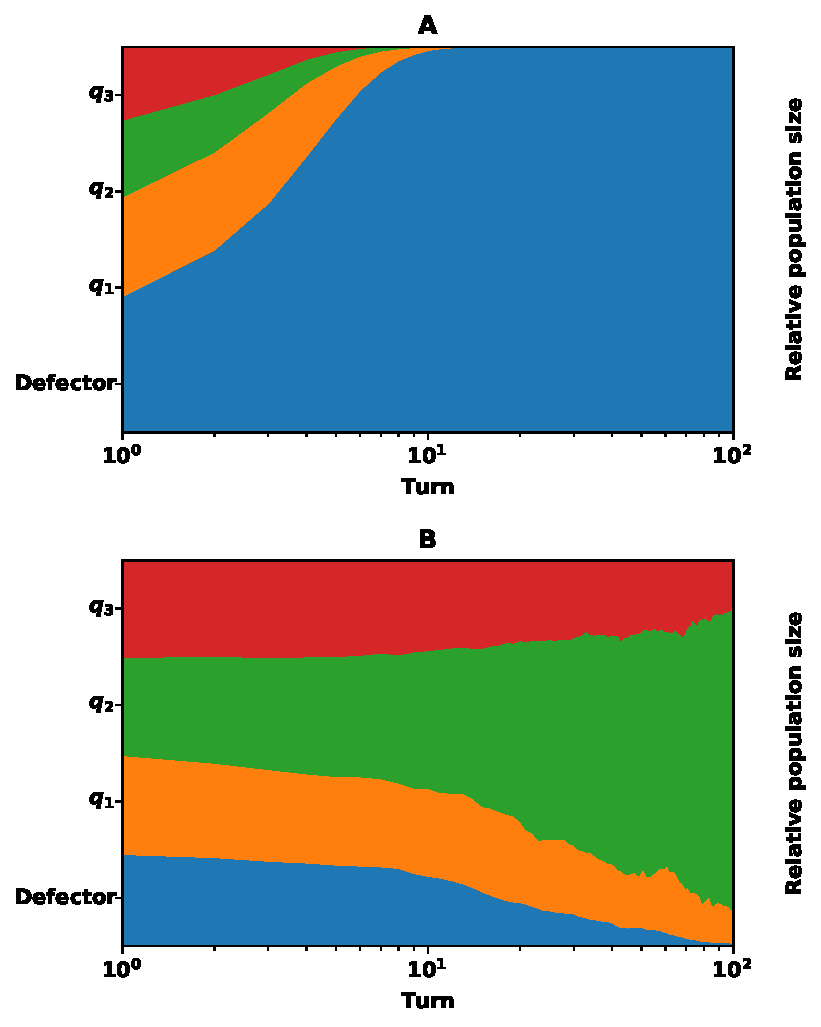
\includegraphics[width=.4\linewidth]{Figure_4.pdf}
    \caption{A. For \(q_{1}=(0.22199, 0.87073, 0.20672, 0.91861)\),
    $q_{2}=(0.48841, 0.61174, 0.76591, 0.51842)$ and
    $q_{3}=(0.2968, 0.18772, 0.08074, 0.73844)$, Equation~(\ref{eq:defection_condition_one}) and
    Equation~(\ref{eq:defection_condition_two}) hold and Defector takes over the
    population. B. For $q_{1}=(0.96703, 0.54723, 0.97268, 0.71482)$,
    $q_{2}=(0.69773, 0.21609, 0.97627, 0.0062)$ and
    $q_{3}=(0.25298, 0.43479, 0.77938, 0.19769)$, Equation~(\ref{eq:defection_condition_one}) fails
    and Defector does not take over the population.
    These results have been obtained by using~\cite{axelrodproject} an open
    source research framework for the study of the IPD.}\label{fig:stability_of_defection}
\end{figure}

\section{Best response memory-one strategy in environments with noise}\label{appendix:noise}

Consider an environment where there is a probability \(p_n\) that a players actions are
executed wrong. This is referred to as the probability of noise.
Two memory-one opponents \(p \in \R_{[0, 1]} ^ 4\) and \(q \in \R_{[0, 1]} ^ 4\)
are now given by:

\[p = (p_1 (1 - p_n), p_2 (1 - p_n), p_3 (1 - p_n), p_4 (1 - p_n))\]

and

\[q = (q_1 (1 - p_n), q_2 (1 - p_n), q_3 (1 - p_n), q_4 (1 - p_n)).\]

Following a similar approach to that of Theorem~1 it
can be shown that the utility \(u_q(p)\) is give by:

\begin{equation}\label{eq:utility_with_noise}
    u_q(p) = \frac{\frac{1}{2}pQp^T + cp + a}
                {\frac{1}{2}p\bar{Q}p^T + \bar{c}p + \bar{a}},
\end{equation}
where \(Q, \bar{Q}\) \(\in \R^{4\times4}\) are square matrices defined by the
transition probabilities of the opponent \(q_1, q_2, q_3, q_4\) as follows:

\begin{center}
\begin{equation*}
\resizebox{\linewidth}{!}{\arraycolsep=2.5pt%
\boldmath\(
Q = \left[\begin{matrix}0 & - p_{n}^{3} \left(q_{1} - q_{3}\right) \left(P p_{n} q_{2} - P - T p_{n} q_{4}\right) & p_{n}^{4} \left(q_{1} - q_{2}\right) \left(P q_{3} - S q_{4}\right) & p_{n}^{3} \left(q_{1} - q_{4}\right) \left(S p_{n} q_{2} - S - T p_{n} q_{3}\right)\\- p_{n}^{3} \left(q_{1} - q_{3}\right) \left(P p_{n} q_{2} - P - T p_{n} q_{4}\right) & 0 & p_{n}^{3} \left(q_{2} - q_{3}\right) \left(P p_{n} q_{1} - P - R p_{n} q_{4}\right) & - p_{n}^{3} \left(q_{3} - q_{4}\right) \left(R p_{n} q_{2} - R - T p_{n} q_{1} + T\right)\\p_{n}^{4} \left(q_{1} - q_{2}\right) \left(P q_{3} - S q_{4}\right) & p_{n}^{3} \left(q_{2} - q_{3}\right) \left(P p_{n} q_{1} - P - R p_{n} q_{4}\right) & 0 & p_{n}^{3} \left(q_{2} - q_{4}\right) \left(R p_{n} q_{3} - S p_{n} q_{1} + S\right)\\p_{n}^{3} \left(q_{1} - q_{4}\right) \left(S p_{n} q_{2} - S - T p_{n} q_{3}\right) & - p_{n}^{3} \left(q_{3} - q_{4}\right) \left(R p_{n} q_{2} - R - T p_{n} q_{1} + T\right) & p_{n}^{3} \left(q_{2} - q_{4}\right) \left(R p_{n} q_{3} - S p_{n} q_{1} + S\right) & 0\end{matrix}\right]\)},
\end{equation*}
\begin{equation*}\label{eq:q_bar_matrix}
\resizebox{\linewidth}{!}{\arraycolsep=2.5pt%
\boldmath\(
\bar{Q} =  \left[\begin{matrix}0 & - p_{n}^{3} \left(q_{1} - q_{3}\right) \left(p_{n} q_{2} - p_{n} q_{4} - 1\right) & p_{n}^{4} \left(q_{1} - q_{2}\right) \left(q_{3} - q_{4}\right) & p_{n}^{3} \left(q_{1} - q_{4}\right) \left(p_{n} q_{2} - p_{n} q_{3} - 1\right)\\- p_{n}^{3} \left(q_{1} - q_{3}\right) \left(p_{n} q_{2} - p_{n} q_{4} - 1\right) & 0 & p_{n}^{3} \left(q_{2} - q_{3}\right) \left(p_{n} q_{1} - p_{n} q_{4} - 1\right) & p_{n}^{4} \left(q_{1} - q_{2}\right) \left(q_{3} - q_{4}\right)\\p_{n}^{4} \left(q_{1} - q_{2}\right) \left(q_{3} - q_{4}\right) & p_{n}^{3} \left(q_{2} - q_{3}\right) \left(p_{n} q_{1} - p_{n} q_{4} - 1\right) & 0 & - p_{n}^{3} \left(q_{2} - q_{4}\right) \left(p_{n} q_{1} - p_{n} q_{3} - 1\right)\\p_{n}^{3} \left(q_{1} - q_{4}\right) \left(p_{n} q_{2} - p_{n} q_{3} - 1\right) & p_{n}^{4} \left(q_{1} - q_{2}\right) \left(q_{3} - q_{4}\right) & - p_{n}^{3} \left(q_{2} - q_{4}\right) \left(p_{n} q_{1} - p_{n} q_{3} - 1\right) & 0\end{matrix}\right]\)}.
\end{equation*}
\end{center}

\(c \text{ and } \bar{c}\) \(\in \R^{4 \times 1}\) are similarly defined by:

\begin{equation}\label{eq:q_matrix_numerator}
\resizebox{0.7\linewidth}{!}{\arraycolsep=2.5pt%
\boldmath\(c = \left[\begin{matrix}p_{n}^{2} q_{1} \left(P p_{n} q_{2} - P - T p_{n} q_{4}\right)\\- p_{n} \left(p_{n} q_{3} - 1\right) \left(P p_{n} q_{2} - P - T p_{n} q_{4}\right)\\- p_{n}^{2} \left(P p_{n} q_{1} q_{2} - P p_{n} q_{2} q_{3} - P q_{2} + P q_{3} - R p_{n} q_{2} q_{4} + S p_{n} q_{2} q_{4} - S q_{4}\right)\\- p_{n} \left(R p_{n}^{2} q_{2} q_{4} - R p_{n} q_{4} - S p_{n}^{2} q_{2} q_{4} + S p_{n} q_{2} + S p_{n} q_{4} - S - T p_{n}^{2} q_{1} q_{4} + T p_{n}^{2} q_{3} q_{4} - T p_{n} q_{3} + T p_{n} q_{4}\right)\end{matrix}\right]\),}
\end{equation}
\begin{equation}\label{eq:q_matrix_denominator}
\resizebox{0.4\linewidth}{!}{\arraycolsep=2.5pt%
\boldmath\(\bar{c} = \left[\begin{matrix}p_{n}^{2} q_{1} \left(p_{n} q_{2} - p_{n} q_{4} - 1\right)\\- p_{n} \left(p_{n} q_{3} - 1\right) \left(p_{n} q_{2} - p_{n} q_{4} - 1\right)\\- p_{n}^{2} \left(p_{n} q_{1} q_{2} - p_{n} q_{2} q_{3} - q_{2} + q_{3} - q_{4}\right)\\p_{n} \left(p_{n}^{2} q_{1} q_{4} - p_{n}^{2} q_{3} q_{4} - p_{n} q_{2} + p_{n} q_{3} - p_{n} q_{4} + 1\right)\end{matrix}\right]\),
}
\end{equation}
and the constant terms \(a, \bar{a}\) are defined as \(a = P + p_{n} \left(- P q_{2} + T q_{4}\right)\) and
\(\bar{a} = p_{n} \left(- q_{2} + q_{4}\right) + 1\).

\bibliographystyle{plain}
\bibliography{bibliography.bib}

\end{document}